\begin{tikzpicture}
\node[anchor=south west,inner sep=0] at (-.05,0) {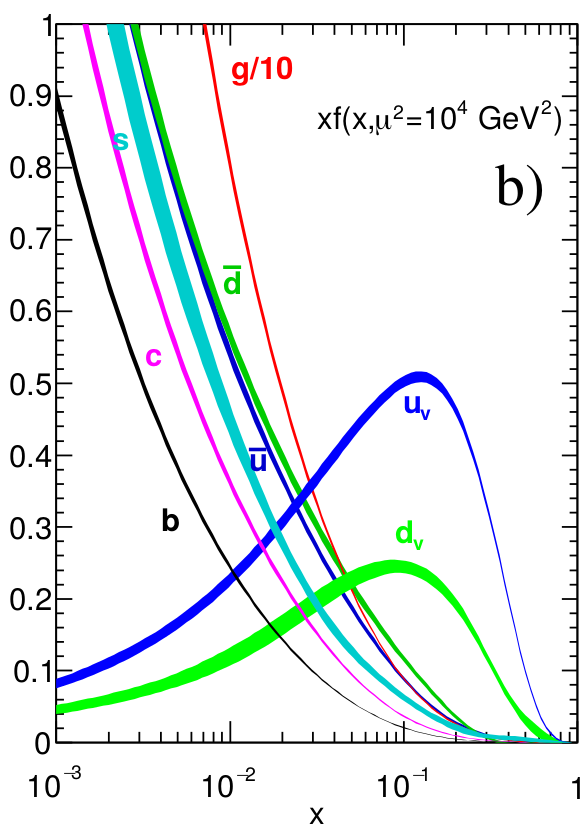
\includegraphics[width=5cm]{\PhDthesisdir/plots_and_images/from_PDG_booklet_2018/parton_pdf_10000_GeV2.png}};

% masks
\fill [white] (0,0) rectangle (5,.75);
\fill [white] (0,0) rectangle (.425,7);
\fill [white] (2.6,6.3) -- (2.6,5.9) -- (4.1,5.2) -- (4.7,5.2) -- (4.7,5.8) -- (4.8,6) -- (4.8,6.2) -- (4.7,6.3);

% X axis
\foreach \pos/\val in {-3/e-3,-2/e-2,-1/e-1,0/1}{
\draw ({4.9+(4.9-.45)*(\pos)/(3)}, .4) node {\footnotesize \num{\val}\vphantom{ÀQg}};
}
\draw (2.7, .2) node {\normalsize $x$};

% Y axis
\foreach \val in {0,0.1,0.2,0.3,0.4,0.5,0.6,0.7,0.8,0.9,1}{
\draw (.5, {.75+\val*(6.9-.75)}) node [left] {\footnotesize \num{\val}};
}

\draw (4.9,6) node [left] {\scriptsize $x \, f(x, \mu^2=\SI{e4}{\GeV^2})$};

\end{tikzpicture}
